\documentclass[10pt,a4paper]{article}
\usepackage[utf8]{inputenc}
\usepackage[a4paper,margin=2.2cm]{geometry}
\usepackage{amsmath,amssymb}
\usepackage{booktabs,graphicx,enumitem,float}
\usepackage[font=small,labelfont=bf,labelsep=period]{caption}
\usepackage[colorlinks=true,urlcolor=black,linkcolor=black]{hyperref}
\setlength{\parindent}{0pt}\setlength{\parskip}{4pt plus 1pt}
\setlist{nosep,leftmargin=1.5em,itemsep=2pt}
\newcommand{\dg}{^{\circ}}
\newcommand{\ci}[2]{$[#1,\,#2]$}
\newcommand{\dsq}{\mathrm{deg}^2}
\newcommand{\res}[1]{\textbf{Result #1.}}
\newcommand{\hyp}{\emph{Hypotheses.} }
\newcommand{\stat}{\emph{Statistic.} }
\newcommand{\rul}{\emph{Rule.} }
\newcommand{\dat}{\emph{Data.} }
\newcommand{\outc}{\emph{Outcome.} }

\begin{document}

\begin{center}
{\Large\bfseries Systematic biases in spatial working memory:\\[2pt] a reanalysis of open data with pre-specified tests}\\[6pt]
{\small Nikita Filippov. October 2026. Code: \texttt{https://github.com/stockman2/schizo-study-v1.git}}
\end{center}

\textbf{Summary.} This document is a worked example of a reanalysis of open data. We reanalysed the data
of Stein, Barbosa et al.\ (2020) on single-item spatial working memory. Every decision rule was fixed before the
corresponding computation, every method was first run on synthetic data with a known answer, and a part of the
data was reserved for confirmation. The main results reproduce known findings; we do not claim that they are
new (see ``Relation to prior work''). About half of the error variance is a systematic bias that depends on
the target location. Its main component is an attraction toward the diagonals. The strength of this attraction
is proportional to the random variance, as in the category adjustment model. A second group of biases grows
at an approximately constant rate during the delay; the attraction toward the previous target belongs to this
group. A model with a drift during the delay predicts the correct size of the location dependence of the
random variance. A model with a single correction at the time of the response predicts an effect that is too
large by a factor of about two. In patients with schizophrenia the biases of the second group are smaller;
this statement is exploratory.

\textbf{How to read this document.} Each result is stated in the same form: the hypotheses that were
compared, the statistic, the decision rule, the data, and the outcome. Every decision rule was written in the
analysis script before the corresponding computation. Section~2 defines all quantities.

\section*{Relation to prior work}

The phenomena analysed here are known. We list the correspondences.
\begin{itemize}
\item \emph{Category adjustment model} (Huttenlocher, Hedges and Duncan, 1991). Estimates of the location of a
dot in a circle are biased away from the horizontal and vertical axes, toward the centres of the quadrants.
The estimate is a weighted mean of an inexact memory and the centre of the category. The weight of the category
increases with the uncertainty, for example with the delay. Results 1 and 2 reproduce this. Our hypothesis (H1)
is the weighting rule of this model, and our model R is a model of this type.
\item \emph{Dynamic field theory} (Spencer and Hund, 2002, 2003; Schutte and Spencer, 2002, 2009). In this
neural field model the memory drifts during the delay. This literature separates geometric biases away from
reference axes, drift during the delay, and biases toward previously used locations. Our classes U and D
(Section~4) are close to this separation. Result~5 is close to the drift toward previous locations reported
there.
\item \emph{Attractor dynamics with drift and diffusion} (Panichello et al., 2019). Errors in colour memory
were described by diffusion together with a drift toward attractor states. The attraction is stronger when
the noise is larger. Our model D is of this type.
\item \emph{Schizophrenia.} Badcock et al.\ (2008) reported that imprecise spatial memory in patients is
accompanied by a larger bias from category-level representations. Stein et al.\ (2020) reported that the
attraction toward the previous target is absent in patients. In the present data the category bias is not
larger in patients (Result~8).
\item \emph{Efficient coding} (Wei and Stocker, 2015) is the alternative hypothesis in Result~10.
\end{itemize}

\textbf{What this document adds.} (i)~A procedure: pre-specified rules, validation on synthetic data, and a
held-out part of the data. (ii)~A quantitative test of the weighting rule over delays within participants,
with a replication. (iii)~Relation (\ref{two}): a gradual attraction and a single correction of the same size
differ by a factor of two in their effect on the local variance. This gives a test between the two types of
model. We did not find this test in the works that we read; our search was not exhaustive. (iv)~An exploratory
comparison of the late drift between patients and controls.

\section*{1. Task and data}

\textbf{Task.} A dot is shown for $0.25$~s on a circle around the fixation point. After a delay
$t\in\{0,1,3\}$~s the participant reports the location of the dot with the mouse. For $t=0$ the dot remains
visible until the response begins; hence there is no memory interval at $t=0$.

\textbf{Samples.} \emph{Baseline sessions:} $52$ participants ($19$ healthy controls, $17$ patients with
schizophrenia, $16$ patients with anti-NMDAR encephalitis), $52\,394$ trials after the exclusion criteria of
the original study (this number equals the published number). \emph{Post sessions} (3--12 months later): $22$
of these participants ($8$ controls, $14$ patients with encephalitis), $23\,356$ trials.

\textbf{Roles of the samples.} A statement is called \emph{exploratory} if it was found in the baseline
sessions without a rule fixed in advance. A statement is called \emph{confirmed} if it satisfied a rule fixed
in advance on data that had not been used to formulate it. The post sessions were reserved for confirmation.
Each quantity was computed in the post sessions only once.

\section*{2. Definitions}

Angles are measured in degrees in the coordinates of the data file. The \emph{cardinal axes} are the
directions $0\dg$, $90\dg$, $180\dg$, $270\dg$. The \emph{diagonals} are the directions $45\dg$, $135\dg$,
$225\dg$, $315\dg$ (Fig.~1a).

\begin{figure}[H]\centering
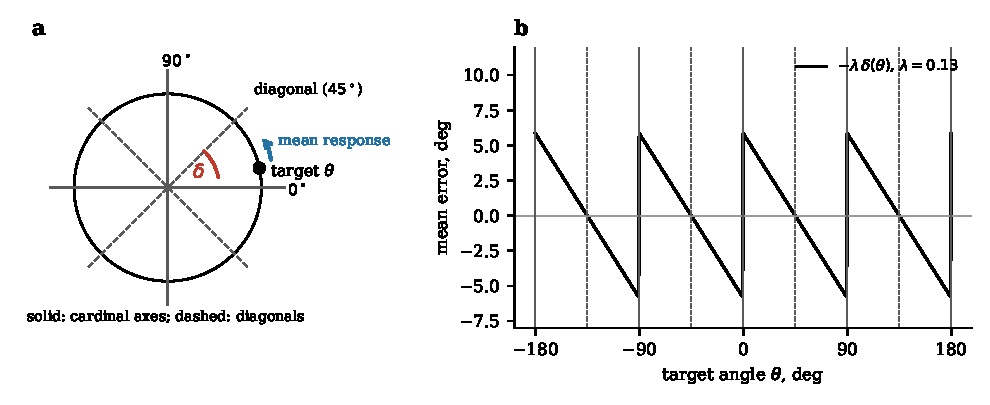
\includegraphics[width=0.78\textwidth]{figE0.pdf}
\caption{(a)~Geometry. The signed distance $\delta$ from the target to the nearest diagonal; an attraction
toward the diagonal moves the mean response as shown. (b)~The mean error $-\lambda\,\delta(\theta)$ produced by
an attraction with coefficient $\lambda$.}
\end{figure}

For a trial with target angle $\theta$ and response angle $r$, the \emph{error} is $\varepsilon=r-\theta$
(wrapped to $[-180\dg,180\dg)$). Let $d$ be the angle from the current target to the target of the previous
trial. All quantities below are computed for each participant and each delay $t$ separately, after the mean
error is subtracted.

\begin{itemize}
\item \emph{Serial bias} $\beta$. We fit $\varepsilon=\beta\,G(d)$ by least squares, where $G$ is the first
derivative of a Gaussian with width $0.8$~rad, normalised to maximum $1$ (the function used in the original
study). $\beta>0$ means that the response is attracted toward the previous target. The term $\beta\,G(d)$ is
then subtracted.
\item \emph{Bias map and random variance.} The bias map is the mean error as a function of $\theta$. Its
variance $V_{\mathrm{map}}$ is estimated without bias from two disjoint halves of the trials ($24$ bins of
$15\dg$; the product of the two half-means is averaged over bins). The \emph{random variance} is
$V=\operatorname{Var}\varepsilon-V_{\mathrm{map}}$.
\item \emph{Attraction coefficient} $\lambda$. Let $\delta(\theta)\in[-45\dg,45\dg)$ be the signed distance
from $\theta$ to the nearest diagonal. We fit
$\varepsilon=-\lambda\,\delta(\theta)+a_1\sin\theta+b_1\cos\theta+a_2\sin2\theta+b_2\cos2\theta+c$.
$\lambda=0.13$ means that the mean response moves $13\%$ of the distance from the target to the diagonal
(Fig.~1b).
\item \emph{Shift in one direction.} The first harmonic $a_1\sin\theta+b_1\cos\theta=A_1\sin(\varphi_1-\theta)$
corresponds to a displacement of all remembered locations toward the direction $\varphi_1$ with amplitude
$A_1$.
\item \emph{Attraction toward the axis $0\dg$--$180\dg$.} The second harmonic equals $A_2\sin2(\varphi_2-\theta)$.
We define $s_2$ as its component for $\varphi_2=0\dg$; $s_2>0$ means attraction toward the axis
$0\dg$--$180\dg$.
\end{itemize}

\textbf{Group statistics.} A group value is the mean over participants. Intervals are $95\%$ bootstrap
intervals ($2000$ resamples of participants) unless stated otherwise. A prediction that is computed from group
values is recomputed in every resample.

\textbf{Compatibility rule.} Several tests compare an observed value with a prediction. We call a hypothesis
\emph{compatible} with the data if the interval of the difference (observed minus predicted) contains zero.
A hypothesis is \emph{accepted} if it is the only compatible hypothesis among those compared.

\textbf{Validation of methods.} Before each computation on the data, the script was run on synthetic data
that were generated under each of the compared hypotheses. A script was used only after it had returned the
correct answer for every synthetic data set.

\section*{3. Results on the data}

\res{1} \emph{About half of the error variance is systematic.}

\stat The share of $V_{\mathrm{map}}$ in the growth of the total variance between $t=1$ and $t=3$~s.\\
\rul Share $\le0.2$: the growth is random. Share $\ge0.5$: the growth is systematic. Otherwise: both.\\
\dat Baseline sessions.\\
\outc In controls the total variance is $14.5$, $38.8$, $57.2~\dsq$ at $t=0,1,3$~s, and $V_{\mathrm{map}}$ is
$4.7$, $16.7$, $27.0~\dsq$. The share is $0.56$ \ci{0.42}{0.67} in controls, $0.52$ in patients with
schizophrenia, $0.57$ in patients with encephalitis. The maps of different participants are correlated
($r\approx0.5$--$0.6$). Harmonics $4$, $8$, $12$ contain $61\%$ of $V_{\mathrm{map}}$: the responses are
attracted toward the diagonals.

\res{2} \emph{The attraction toward the diagonals is proportional to the random variance.}

\hyp (H1) The attraction follows the uncertainty (the weighting rule of the category adjustment model):
\begin{equation}
\lambda(t)\bigl(1-\lambda(t)\bigr)=V(t)/V_p .
\label{law}
\end{equation}
(H2) The trace moves toward the diagonal at a constant relative rate:
\begin{equation}
1-\lambda(t)=\bigl(1-\lambda(0)\bigr)e^{-kt}.
\label{rate}
\end{equation}
\stat The observed $\lambda(3)$ and two predictions computed from $t=0$ and $t=1$. Under (H1):
$\lambda(3)\bigl(1-\lambda(3)\bigr)=\lambda(1)\bigl(1-\lambda(1)\bigr)\,V(3)/V(1)$. Under (H2):
$1-\lambda(3)=(1-\lambda(0))\bigl[(1-\lambda(1))/(1-\lambda(0))\bigr]^3$.\\
\rul Compatibility rule (Section~2).\\
\dat Baseline sessions (first test); post sessions (replication).\\
\outc Table~1 and Fig.~2a. (H2) is not compatible and (H1) is compatible in both samples. A second test in the
post sessions: the ratio $\lambda(1-\lambda)/V$ is constant over the delays (Fig.~2b). The rule required
that the intervals of the ratios of consecutive delays contain $1$; they are $0.95$ \ci{0.80}{1.27} and
$1.03$ \ci{0.88}{1.22}. The constant is $V_p\approx310$--$320~\dsq$.

\begin{table}[H]\centering\small
\caption{Attraction coefficient at $t=3$~s: observation and two predictions.}
\begin{tabular}{lccc}\toprule
 & Observed & Prediction (H2) & Prediction (H1)\\\midrule
Baseline, $n=52$ & 0.132 \ci{0.117}{0.147} & 0.192 \ci{0.169}{0.216} & 0.127 \ci{0.107}{0.149}\\
Post, $n=22$ & 0.125 \ci{0.102}{0.152} & 0.198 \ci{0.158}{0.237} & 0.121 \ci{0.089}{0.159}\\\bottomrule
\end{tabular}
\end{table}

\res{3} \emph{A shift in one direction has a constant part and a part that follows the random variance.}

\hyp For the growth of the shift between $1$ and $3$~s: (H1) the increment is proportional to the increment
of $V$; (H2) the shift grows at a constant rate.\\
\stat Let $p_1(t)$ be the component of the first harmonic in the direction $-85\dg$ (this direction was
found in the exploratory analysis and was then fixed). The observed increment $p_1(3)-p_1(1)$ is compared
with $[p_1(1)-p_1(0)]\,[V(3)-V(1)]/[V(1)-V(0)]$ under (H1) and with $2\,[p_1(1)-p_1(0)]$ under (H2).\\
\rul Compatibility rule. In addition, the direction is confirmed if its interval lies in $[-135\dg,-45\dg]$.\\
\dat Exploration: baseline sessions. Confirmation: post sessions.\\
\outc The direction is $-89\dg$ \ci{-107\dg}{-70\dg}. The amplitude is $1.3\dg$ at $t=0$ and $2.5\dg$ at
$t=3$~s. The observed increment is $0.23\dg$. Under (H1) the prediction is $0.22\dg$ (difference $0.01\dg$
\ci{-0.54}{0.62}). Under (H2) it is $1.87\dg$ (difference $-1.64\dg$ \ci{-2.75}{-0.59}). (H1) is accepted.

\res{4} \emph{The attraction toward the axis $0\dg$--$180\dg$ is a late drift.}

\hyp The mean of $s_2$ does not change during the first second and grows afterwards. This is the opposite of
(H1): $V$ grows mainly during the first second (Table~2).\\
\stat The early increment $F=s_2(1)-s_2(0)$ and the late rate $L=[s_2(3)-s_2(1)]/2$.\\
\rul Confirmed if the interval of $L$ lies above zero and the interval of $F-L$ lies below zero.\\
\dat Exploration: baseline sessions. Confirmation: post sessions.\\
\outc Post sessions: $L=0.45\dg$/s \ci{0.23}{0.67}, $F=-0.13\dg$ \ci{-0.70}{0.42}, $F-L=-0.58\dg$
\ci{-1.16}{-0.01} (Fig.~2c). Exploration: $L=0.52\dg$/s \ci{0.39}{0.67}. The statement is confirmed; the upper
bound of $F-L$ is close to zero.

\res{5} \emph{The attraction toward the previous target grows faster than the random variance.}

\hyp For the growth of $\beta$: (H1) the increment is proportional to the increment of $V$; (H2) $\beta$
grows at a constant rate.\\
\stat The observed $\beta(3)$ is compared with $\beta(0)+[\beta(1)-\beta(0)]\,[V(3)-V(0)]/[V(1)-V(0)]$ under
(H1) and with $\beta(0)+3\,[\beta(1)-\beta(0)]$ under (H2).\\
\rul Confirmed if the interval of the difference between the observation and the prediction of (H1) lies
above zero.\\
\dat Post sessions ($\beta$ had not been computed there before).\\
\outc $\beta=-0.29\dg$, $+0.34\dg$, $+2.09\dg$ at $t=0,1,3$~s. Under (H1) the prediction is $0.65\dg$; the
difference is $+1.44\dg$ \ci{0.80}{2.05}. Under (H2) the prediction is $1.59\dg$; the difference is $+0.51\dg$
\ci{-0.63}{1.57}. The statement is confirmed, and (H2) is compatible.

\res{6} \emph{Individual bias fields are stable.}

\stat The correlation, across participants, between the pre and post sessions of the individual components of
the first harmonic and of the second harmonic (the group mean is subtracted), $t=1$~s.\\
\rul Confirmed if the lower bound of the interval is above zero.\\
\outc $r=0.52$ \ci{0.15}{0.77} for the first harmonic and $r=0.69$ \ci{0.51}{0.87} for the second harmonic.

\res{7} \emph{The random variance is larger near the cardinal axes than near the diagonals, and the difference
grows with the delay.}

\stat The ratio of the residual variance for targets within $15\dg$ of an axis to the residual variance for
targets within $15\dg$ of a diagonal.\\
\rul Confirmed if the interval of the difference of the ratio between $t=3$ and $t=0$~s lies above zero.\\
\dat Exploration: baseline sessions (ratio $1.15$, $1.37$, $1.69$ at $t=0,1,3$~s). Confirmation: post
sessions.\\
\outc The difference is $0.35$ \ci{0.05}{0.71}. In these ratios the residual was computed after the sawtooth
$-\lambda\delta$ was removed. If a flexible map (harmonics $1$--$12$) is removed instead, the logarithm of the
ratio is $0.24$ \ci{0.17}{0.32} at $1$~s and $0.37$ \ci{0.25}{0.48} at $3$~s (baseline sessions).

\begin{figure}[H]\centering
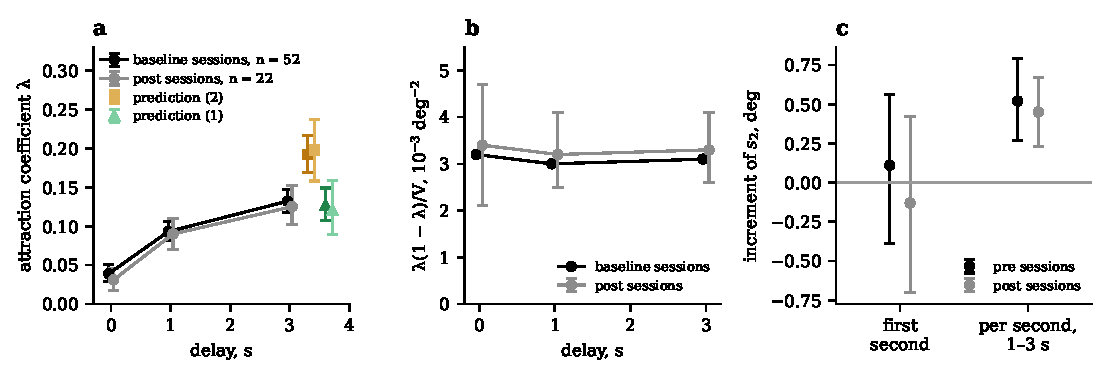
\includegraphics[width=\textwidth]{figE1.pdf}
\caption{(a)~Attraction coefficient $\lambda$ and the two predictions for $t=3$~s (prediction~(1) is (H1),
prediction~(2) is (H2)). (b)~The ratio in (\ref{law}) at the three delays; intervals were not computed for the
baseline sessions. (c)~Increment of $s_2$ in the same $22$ participants in two sessions.}
\end{figure}

\section*{4. Two classes of biases}

Results 2--5 separate the biases into two classes (Table~2).

\textbf{Class U} (the bias follows the uncertainty): the attraction toward the diagonals and the shift in one
direction. Their increments are proportional to the increments of $V$. Most of the growth occurs during the
first second.

\textbf{Class D} (drift): the attraction toward the axis $0\dg$--$180\dg$ and the attraction toward the
previous target. Their growth between $1$ and $3$~s is larger than the growth predicted from $V$.

This distinction is close to the distinction between geometric biases and delay- or experience-dependent
biases in the literature on the dynamic field theory.

\begin{table}[H]\centering\small
\caption{Growth of each component in the post sessions ($n=22$). The unit is $\dsq$ for $V$ and degrees for
the other components; $\lambda$ is dimensionless.}
\begin{tabular}{lccl}\toprule
Component & Increment, $0\to1$~s & Increment, $1\to3$~s & Class\\\midrule
Random variance $V$ & 15.9 & 8.0 & ---\\
Attraction toward diagonals, $\lambda$ & 0.059 & 0.035 & U\\
Shift in one direction, $p_1$ & 0.94 & 0.23 & U\\
Attraction toward axis, $s_2$ & $-0.13$ & 0.90 & D\\
Attraction toward previous target, $\beta$ & 0.62 & 1.76 & D\\\bottomrule
\end{tabular}
\end{table}

\res{8} \emph{In patients with schizophrenia the class D biases are smaller (exploratory).}

\hyp The late drift toward the axis is smaller in patients with schizophrenia than in controls. (The absence
of the attraction toward the previous target in these patients is the published result of the original
study.)\\
\stat The late rate $L$ (Result~4) of each participant; the difference of the group means, controls minus
patients.\\
\rul Confirmed if the interval of the difference lies above zero.\\
\dat Baseline sessions. These data had been inspected before the rule was written. No independent sample of
patients was available.\\
\outc $L=0.60\dg$/s \ci{0.49}{0.72} in controls and $0.34\dg$/s \ci{0.09}{0.58} in patients; the difference
is $0.26\dg$/s \ci{0.01}{0.55}. The rule is satisfied; the lower bound is close to zero. For comparison, the
late increment of $\beta$ is $+2.04\dg$ \ci{1.44}{2.76} in controls and $+0.11\dg$ \ci{-0.71}{0.86} in
patients. Class U is not reduced: $V_{\mathrm{map}}$ at $3$~s is $27.0$, $26.3$, $24.3~\dsq$ in the three
groups.

We state the following \textbf{hypothesis} for future tests: \emph{in schizophrenia the biases of class D are
reduced and the biases of class U are preserved.} Badcock et al.\ (2008) reported a larger category bias in
patients; the present data do not show this. A further test was not informative: the correlation, across participants,
between the late increment of $\beta$ and $L$ is $0.02$ \ci{-0.28}{0.30}, but the split-half reliabilities
of these two individual quantities are $0.27$ and $-0.12$.

\section*{5. A differential model for class U}

\textbf{Model D.} Let $x$ be the location of the memory trace. We assume
\begin{equation}
dx=-\frac{D(t)}{V_*}\,g(x)\,dt+\sqrt{2D(t)}\,dW ,
\label{sde}
\end{equation}
where $g$ is the shape of the attraction ($g=0$ on the diagonals and on the axes), $D(t)$ is the noise
intensity, and $W$ is a Wiener process. The drift is proportional to the noise intensity. Models with diffusion and a drift toward attractor
states were fitted to colour memory by Panichello et al.\ (2019). Let $\tau(t)=\int_0^tD(s)\,ds$. For one well with $g(x)=x$,
\begin{equation}
1-\lambda=e^{-\tau/V_*},\qquad V=V_*\,\lambda\,(2-\lambda).
\end{equation}
For small $\lambda$ this coincides with (\ref{law}) with $V_p=2V_*$. For $\lambda\le0.13$ the two forms
cannot be distinguished in the data. The group means give $V_*\approx150~\dsq$, and $D\approx9.5~\dsq$/s
during the first second and $D\approx2.8~\dsq$/s afterwards.

\textbf{Model R} (a model of the category adjustment type). The trace diffuses without drift and has variance $V_{\mathrm{mem}}$ at the end of the
delay. The response is $m-\lambda\,g(m)$, where $m$ is the final location of the trace and
$\lambda=V_{\mathrm{mem}}/(V_{\mathrm{mem}}+V_p)$.

\textbf{Difference between the models.} Let $s(x)=g'(x)$. To first order in $\lambda$,
\begin{equation}
V_{\mathrm D}(x)\approx2\tau\bigl(1-\lambda\,s(x)\bigr),\qquad
V_{\mathrm R}(x)\approx2\tau\bigl(1-2\lambda\,s(x)\bigr).
\label{two}
\end{equation}
A gradual attraction changes the local variance half as much as a single correction of the same size. Both
models reproduce Result~2. They differ in the dependence of the random variance on the location.

\res{9} \emph{Model R is rejected. Model D predicts the correct size of the effect but is not accepted.}

\hyp Model D against model R.\\
\stat The residual variance in three bands of $|\delta|$: $0$--$15\dg$ (near the diagonal), $15$--$30\dg$
(middle), $30$--$45\dg$ (near the axis), and the ratios of the second and third to the first.\\
\emph{Calibration.} For each participant the well parameter ($V_*$ or $V_p$) was chosen so that the model
reproduces the sum of $\lambda$ over the delays, and the amount of noise at each delay was chosen so that the
model reproduces $V$. Model trials were generated at the target angles of the real trials and were analysed
by the same code. The distribution of the variance over the circle was not used in the calibration.\\
\rul A model is compatible if the $99\%$ interval of the difference between data and model contains zero for
every ratio at $t=1$ and $t=3$~s. A model is accepted if it is the only compatible model.\\
\dat Baseline sessions (main test); post sessions (for reference).\\
\emph{Two rounds.} In the first round $g$ was a sawtooth, $g(x)=\delta(x)$, and only the ratio ``near axis /
near diagonal'' was tested. Model D failed at $t=3$~s. In the second round $g$ was a smooth shape (harmonics
$4$, $8$, $12$) fitted so that the mean bias map of the model equals the measured map, and both ratios were
tested. The second round is a revision after a failed test on data that had been inspected.\\
\outc Table~3 and Fig.~3. Model R overestimates the ratio near the axes by $1.1$--$1.6$ in all eight
comparisons; this agrees with (\ref{two}). Model D with the sawtooth gives the correct level near the axes,
but the middle band does not differ from the band near the diagonal (model $1.00$--$1.02$; data $1.19$ and
$1.26$). Model D with the smooth shape reproduces the middle band ($1.14$ and $1.16$), but the ratio near
the axes is too large at $1$~s and in the post sessions. The data lie between the two variants of model D.
By the rule, neither model is accepted in either round.

\begin{table}[H]\centering\small
\caption{Ratio of the residual variances, near axis / near diagonal. An asterisk indicates that the $99\%$
interval of the difference between data and model does not contain zero.}
\begin{tabular}{llccccc}\toprule
Sample & Delay & Data & D, sawtooth & D, smooth & R, sawtooth & R, smooth\\\midrule
Baseline & 1 s & 1.37 \ci{1.25}{1.50} & 1.32 & 1.60$^*$ & 2.45$^*$ & 2.48$^*$\\
 & 3 s & 1.69 \ci{1.51}{1.88} & 1.44$^*$ & 1.78 & 2.81$^*$ & 2.90$^*$\\\addlinespace
Post & 1 s & 1.22 \ci{1.08}{1.37} & 1.35 & 1.59$^*$ & 2.52$^*$ & 2.44$^*$\\
 & 3 s & 1.25 \ci{1.02}{1.54} & 1.43 & 1.81$^*$ & 2.81$^*$ & 2.67$^*$\\\bottomrule
\end{tabular}
\end{table}

\begin{figure}[H]\centering
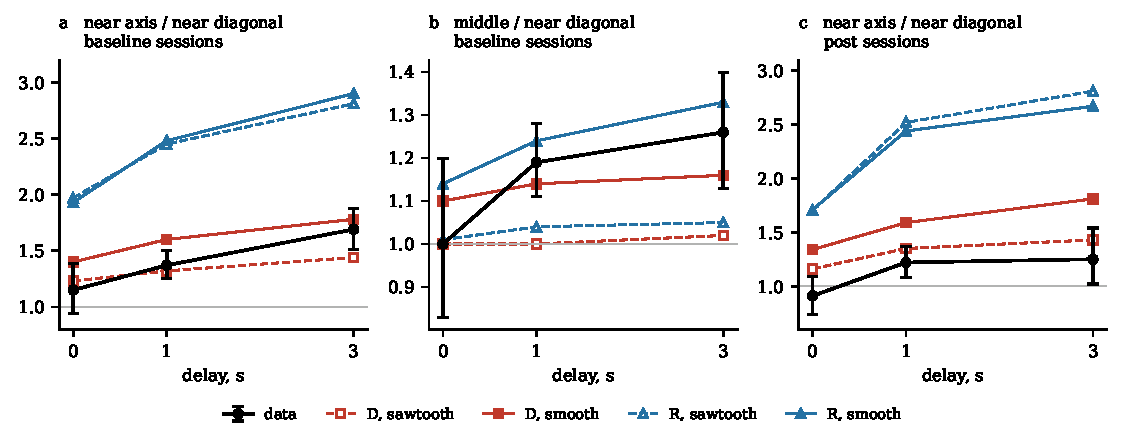
\includegraphics[width=\textwidth]{figE2.pdf}
\caption{Ratios of residual variances: data ($95\%$ intervals) and four model variants. The delay $0$~s is
shown for reference.}
\end{figure}

\section*{6. Scope: perception of orientation and motion direction}

\res{10} \emph{The potential-well picture holds for memory of location and does not hold for the perception
of orientation.}

\hyp In a potential well the responses are attracted toward locations where the random variance is small. An
alternative (efficient coding) predicts that the responses move away from values that are encoded
precisely, that is, toward locations where the random variance is large.\\
\stat For each participant: $\lambda$ (sign: positive toward the diagonals or oblique orientations) and
$m=\ln(\text{variance near the axes}/\text{variance near the diagonals})$, computed after a flexible map is
removed.\\
\rul For each experiment: ``well'' if the intervals of the mean $\lambda$ and of the mean $m$ exclude zero and
the signs are equal; ``opposite'' if both exclude zero and the signs differ; otherwise undecided. For a
stimulus type: the answer is the verdict of at least two thirds of the decided experiments, if at least
three are decided.\\
\dat $30$ open experiments (orientation or motion direction) from the collection of Ozkirli, Chetverikov and
Pascucci (2025); the data of Section~1 for comparison.\\
\outc Location memory (Section~1 data): ``well'' at both delays ($m=0.24$ and $0.37$). Orientation ($22$
experiments): $\lambda>0$ in $19$ experiments ($0.07$--$0.20$, the same range as in Result~2), but $2$
experiments are ``well'', $5$ are ``opposite'', and $15$ are undecided; the verdict by the rule is
``opposite''. Motion direction ($8$ experiments): $2$ are ``well'' and none is ``opposite''; fewer than
three are decided. The two ``well'' experiments are working memory experiments.

\section*{7. Statements that were not confirmed}

\begin{itemize}
\item \emph{Alignment of individual axes.} In the baseline sessions the individual axis of the second harmonic
lies within $22.5\dg$ of $0\dg$ or $90\dg$ in $38$ of $52$ participants. The rule for the post sessions
required at least $16$ of $22$; the observed number is $13$.
\item \emph{Recovery from encephalitis.} We predicted that $\lambda(1-\lambda)/V$ increases from the pre to
the post session in patients. The change is $+0.0005$ \ci{-0.0003}{0.0011}; the interval contains zero.
\item \emph{Differences between participants.} If (\ref{law}) held across participants with a common $V_p$,
then $\lambda$ and $V$ would be correlated. The rank correlation at $t=1$~s is $0.14$ \ci{-0.15}{0.41}
(reliability of both quantities: $0.96$). Relation (\ref{law}) holds within a participant over time.
\item \emph{Growth law of $V(t)$.} At $t=0$ there is no memory interval, and only two positive delays are
available. Diffusion with an initial loss cannot be distinguished from saturation.
\end{itemize}

\section*{8. Limitations}

\begin{itemize}
\item Three delays give two time intervals.
\item The data do not distinguish an attraction that occurs during the delay from an attraction at the time
of the response whose size increases with the delay; only the two specific variants of model R were rejected.
\item The post sessions contain the same participants as the baseline sessions and no patients with
schizophrenia. All statements about schizophrenia rest on the baseline sessions.
\item The orientation of the screen coordinates is not known to us. Gaze was not recorded. The patients were
medicated.
\item Model D does not contain the class D biases, lapses, or trial-to-trial changes of precision.
\end{itemize}

\section*{9. Predictions for data with longer delays}

\begin{enumerate}
\item In model D the random variance saturates at $V_*$ ($125$--$155~\dsq$). In model R the observed variance
does not exceed $V_p/4$ and then decreases.
\item If the class D biases grow at a constant rate, then at delays of $8$--$20$~s they exceed the class U
biases.
\item In patients with schizophrenia the class D biases are reduced at all delays, and the class U biases
are not.
\end{enumerate}

\section*{Use of AI}

The analysis scripts and the text of this document were prepared with the assistance of a large language model (Claude, Anthropic). Nikita Filippov ran all analyses, checked the results, and is responsible for the content.

\section*{Sources}

{\small
Stein H., Barbosa J., et al. Reduced serial dependence suggests deficits in synaptic potentiation in
anti-NMDAR encephalitis and schizophrenia. \emph{Nat.\ Commun.}\ 11, 4250 (2020). Data:
\texttt{github.com/comptelab/serialNMDA}.

Ozkirli A., Chetverikov A., Pascucci D. Large-scale mega-analysis indicates that serial dependence
deteriorates perceptual decision-making. \emph{Nat.\ Hum.\ Behav.}\ (2025), and the original studies listed
in its data repository.

Huttenlocher J., Hedges L.\,V., Duncan S. Categories and particulars: prototype effects in estimating spatial
location. \emph{Psychol.\ Rev.}\ 98, 352--376 (1991).

Spencer J.\,P., Hund A.\,M. Prototypes and particulars: geometric and experience-dependent spatial categories.
\emph{J.\ Exp.\ Psychol.\ Gen.}\ 131, 16--37 (2002).

Spencer J.\,P., Hund A.\,M. Developmental continuity in the processes that underlie spatial recall.
\emph{Cogn.\ Psychol.}\ (2003).

Schutte A.\,R., Spencer J.\,P. Generalizing the dynamic field theory of the A-not-B error beyond infancy.
\emph{Child Dev.}\ 73, 377--404 (2002).

Schutte A.\,R., Spencer J.\,P. Tests of the dynamic field theory and the spatial precision hypothesis.
\emph{J.\ Exp.\ Psychol.\ Hum.\ Percept.\ Perform.}\ (2009).

Panichello M.\,F., DePasquale B., Pillow J.\,W., Buschman T.\,J. Error-correcting dynamics in visual working
memory. \emph{Nat.\ Commun.}\ 10, 3366 (2019).

Badcock J.\,C., et al. Examining encoding imprecision in spatial working memory in schizophrenia.
\emph{Schizophr.\ Res.}\ (2008).

Wei X.-X., Stocker A.\,A. A Bayesian observer model constrained by efficient coding can explain
`anti-Bayesian' percepts. \emph{Nat.\ Neurosci.}\ 18, 1509--1517 (2015).

Gold J.\,M., et al. Refining the empirical constraints on computational models of spatial working memory in
schizophrenia. \emph{Biol.\ Psychiatry Cogn.\ Neurosci.\ Neuroimaging} 5, 913--922 (2020).

Starc M., Murray J.\,D., et al. Schizophrenia is associated with a pattern of spatial working memory deficits
consistent with cortical disinhibition. \emph{Schizophr.\ Res.}\ 181, 107--116 (2017).
}

\end{document}
